\documentclass[11pt,letterpaper,boxed]{../hmcpsetrhino}
\usepackage[margin=1in]{geometry}
\usepackage{graphicx}
\usepackage{enumerate}
\usepackage{amsthm}
\usepackage{amsmath}

\newcommand{\ds}{\displaystyle}
\newcommand{\half}{\frac{1}{2}}
\newcommand*\Eval[3]{\left.#1\right\rvert_{#2}^{#3}}
\newcommand{\eval}{\biggr\rvert}
\newcommand\Partial[2]{\frac{\partial #1}{\partial #2}}
\newcommand\mat[1]{\underline{\vec {#1}}}
\newcommand\tp[1]{\widetilde {#1}}
\def\EE{{\cal E}}
\def\Lagr{\mathcal{L}}
\def\Ham{\mathcal{H}}

\name{}
\class{Physics 111 Section 1}
\assignment{Problem Set 17}
\duedate{November 21, 2016}

\begin{document}

\problemlist{Oscillations: Springs (Reading: Chapter 11.1 - 11.2, 11.7)}
\textbf{Help:}

\begin{problem}[i]
Spring-mass system with only one wall.

\begin{problem}
\begin{enumerate}[(a)]
\item Find the normal frequencies, $\omega_1$ and $\omega_2$, for the carts shown in Figure 11.15, assuming that $m_1 = m_2$ and $k_1 = k_2$.

\item Find and describe the motion for each of the normal modes in turn.
\end{enumerate}
\[	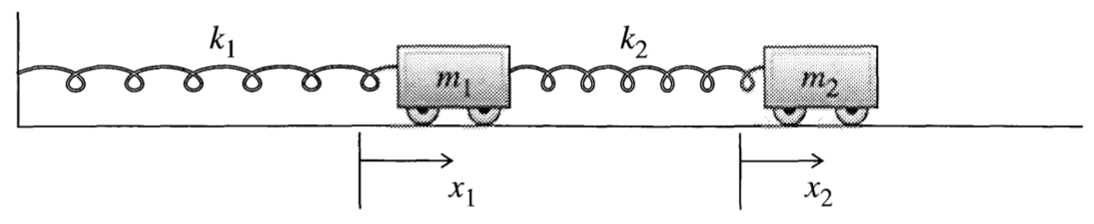
\includegraphics[scale=0.5]{fig1}\]

\end{problem}
\end{problem}
\begin{solution}


\vfill
\end{solution}

\newpage


\begin{problem}[ii]
A little practice with normal coordinates. In part (b), the general result you arrive at should match the result expressed in (11.21).

\begin{problem}
\begin{enumerate}[(a)]
\item Write down the equations of motion (11.2) for the equal mass carts of Section 11.2 with three identical springs. Show that the change of variables to the normal coordinates $\xi_1 = \half (x_1 + x_2)$ and $\xi_2 = \half (x_1 - x_2)$ leads to uncoupled equations for $\xi_1$ and $\xi_2$. 

\item Solve for $\xi_1$ and $\xi_2$ and hence write down the general solution for $x_1$ and $x_2$. (Notice how very simple this procedure is, once you have guessed what the normal coordinates are. For a symmetric system like this, you can sometimes guess the form of $\xi_1$ and $\xi_2$ by considering the symmetry - especially once you have some experience working with normal modes.) 

\end{enumerate}
\end{problem}
\end{problem}
\begin{solution}


\vfill
\end{solution}

\newpage


\begin{problem}[iii]
Damped carts and normal coordinates. In part (c), don't forget to add the homogeneous solution, and in part (e) don't take the "prove" statement literally - strong argument is fine.

\begin{problem}
\begin{enumerate}[(a)]
\item Write down the equations of motion corresponding to (11.2) for the equal-mass carts of Section 11.2 with three identical springs, but with each cart subject to a linear resistive force $-b\vec v$.(same coefficient $b$ for both carts) and with a driving force $F(t) = F_0 \cos \omega t$ applied to cart 1.

\item Show that if you change variables to the normal coordinates $\xi_1 = \half (x_1 + x_2)$ and $\xi_2 = \half (x_1 - x_2)$, the equations of motion for $\xi_1$ and $\xi_2$ are uncoupled.

\item Using the methods of Section 5.5, write down the general solutions. 

\item Assuming $\beta = b/2m \ll \omega_0$, show that $\xi_1$ resonates when $\omega \approx \omega_0 = \sqrt{k /m}$ and likewise $\xi_2$ when $\omega \approx \sqrt{3} \omega_0$. 

\item Prove, on the other hand, that if both carts are driven in phase with the same force $F_0 \cos \omega t$, only $\xi_1$ shows resonance. Explain.

\end{enumerate}
\end{problem}
\end{problem}
\begin{solution}


\vfill
\end{solution}

\newpage


\begin{problem}[ii]
Carts coupled by molasses.

\begin{problem}
Here is a different way to couple two oscillators. The two carts in Figure 11.16 have equal masses $m$ (though different shapes). They are joined by identical but separate springs (force constant $k$) to separate walls. Cart 2 rides in cart 1, as shown, and cart 1 is filled with molasses, whose viscous drag supplies the coupling between the carts.

\begin{enumerate}[(a)]
\item Assuming that the drag force has magnitude $\beta m v$ where $\vec v$ is the relative velocity of the two carts, write down the equations of motion of the two carts using as coordinates $x_1$ and $x_2$, the displacements of the carts from their equilibrium positions. Show that they can be written in matrix form as $\ddot{ \vec x} + \beta \mat D \dot{ \vec x} + {\omega_0}^2 x = 0$, where $\vec x$ is the 2 $\times$ 1 column made up of $x_1$ and $x_2$, $\omega_0 = \sqrt{k/m}$ and $\mat D$ is a certain 2 $\times$ 2 square matrix. 

\item There is nothing to stop you from seeking a solution for the form $\vec x(t) = Re \vec z(t) = \vec a e^{rt}$. Show that you do indeed get two solutions of this form with $r = i \omega_0$ or $r = - \beta + i \omega_1$ where $\omega_1 = \sqrt{{\omega_0}^2 - \beta^2}$. (Assume that the viscous force is weak, so that $\beta < \omega_0$.)

\item Describe the corresponding motions. Explain why one of these modes is damped but the other is not.
\end{enumerate}

\[	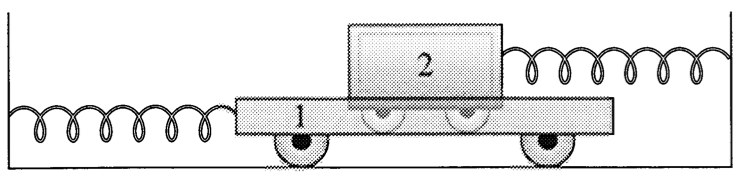
\includegraphics{fig2}\]

\end{problem}
\end{problem}
\begin{solution}


\vfill
\end{solution}


\end{document}
